\documentclass{beamer}

\usepackage{colortbl}
\usepackage{tikz}

\usetheme{Boadilla}

\usetikzlibrary{arrows,positioning}

\tikzstyle{language}=[rectangle,draw=black,thin,
inner sep=3pt, font=\tiny, align=center]

\tikzstyle{compiler}=[rectangle,rounded corners,draw=black,thin,
inner sep=3pt, font=\tiny, align=center]

\tikzstyle{added}=[fill=gray]

\title{Implementation and Evaluation of ZK-PoK}
\author{Boran Car}
\institute{K. U. Leuven}

\begin{document}

\begin{frame}
  \titlepage
\end{frame}

\begin{frame}
  \frametitle{Outline}

  \begin{enumerate}
  \item The Problem
  \item Anonimity
  \item The Goal
  \item Why go to custom framework?
  \item CACE workflow
  \item Custom framework workflow
  \item LLVM
  \item GEZEL
  \item Planning
  \item Custom framework status
  \end{enumerate}
\end{frame}

\begin{frame}
  \frametitle{The Problem}

  \begin{itemize}
  \item Zero Knowledge Proofs of Knowledge
    \begin{itemize}
    \item Prove knowledge of something without actually disclosing it
    \end{itemize}
  \item A base for
    \begin{itemize}
    \item E-petition
    \item E-voting
    \item E-cash
    \item Anonymous credentials (e.g. driver license)
    \end{itemize}
  \end{itemize}
\end{frame}

\begin{frame}
  \frametitle{Anonimity}
  
  \begin{itemize}
  \item Current electronic methods require log-in
    \begin{itemize}
    \item The user has no choice but to give his personal information
    \item ``Big-Brother'' can track you
    \end{itemize}
  \item Current paper methods too slow
    \begin{itemize}
    \item Waste paper
    \item Waste man-hours
      \begin{itemize}
      \item Counting
      \item Processing
      \end{itemize}
    \end{itemize}
  \end{itemize}
\end{frame}

\begin{frame}
  \frametitle{The Goal}

  \begin{itemize}
  \item Proving something without disclosing it is not very simple
    \begin{itemize}
    \item Luckily, there exist some frameworks
    \end{itemize}
  \item The initial goals were:
    \begin{enumerate}
    \item To evaluate existing ZK-PoK frameworks
    \item To implement DAA - Direct Anonymous Attestation
    \end{enumerate}
  \item Later this has changed to:
    \begin{enumerate}
    \item Evaluate existing ZK-PoK frameworks
    \item Implement a custom framework
    \item Implement DAA on top of the custom framework
    \end{enumerate}
  \end{itemize}
\end{frame}

\begin{frame}
  \frametitle{Why go to custom framework?}
  
  \begin{itemize}
  \item Avaiable frameworks not fit for small embedded devices
    \begin{itemize}
    \item CACE - Generated C code polluted with debugging info not easily strippable
    \item ZKPDL - Uses C++ which is not available for all small devices,
interpreter framework
    \end{itemize}
  \item DFG difficult to extract from existing frameworks
    \begin{itemize}
    \item DFG needed for conversion to HDL
    \item Easier optimizations (e.g. intermediate result caching)
    \end{itemize}
  \item Domain specific language fit for cryptographers
  \end{itemize}
\end{frame}

\begin{frame}
  \frametitle{CACE workflow}
  
  \begin{center}
  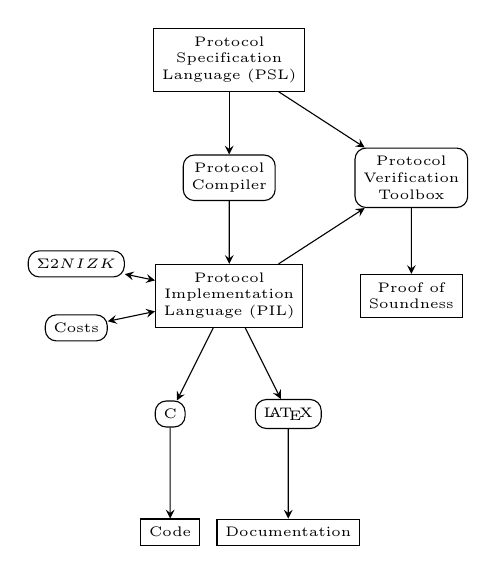
\begin{tikzpicture}[>=stealth]
    \tikzstyle{edge from parent}=[draw,->]
    \node[language] (psl) {Protocol \\ Specification \\ Language (PSL)}
    child {node[compiler] (pc) {Protocol \\ Compiler}
        child {node[language] (pil) {Protocol \\ Implementation \\ Language (PIL)}
            child {node[compiler] (c) {C}
              child {node[language] (code) {Code}}}
            child {node[compiler] (latex) {\LaTeX}
              child {node[language] (doc) {Documentation}}}
          }};

    \node[compiler] (pvt)         [right=of pc,anchor=west]          {Protocol \\ Verification \\ Toolbox}
    child {node[language] {Proof of \\ Soundness}};

    \node[compiler] (sigma) [left=of pil.north west,anchor=center] {$\Sigma 2 N I Z K$};
    \node[compiler] (cost) [left=of pil.south west,anchor=center] {Costs};

    \draw[<->] (sigma) -- (pil);
    \draw[<->] (cost) -- (pil);

    \draw[->] (psl) -- (pvt);
    \draw[->] (pil) -- (pvt);
  \end{tikzpicture}
  \end{center}
\end{frame}

\begin{frame}
  \frametitle{Custom framework}

  \begin{itemize}
  \item Extends CACE (Computer Aided Cryptography Engineering), an European project
  \item Uses LLVM - Low Level Virtual Machine
    \begin{itemize}
    \item A VM Load-Store RISC architecture
      \begin{itemize}
      \item Infinite SSA registers
      \end{itemize}
    \end{itemize}
  \item Allows for
    \begin{itemize}
    \item Interpreted
    \item Compiled
    \item JIT Compiled
    \end{itemize}
  \end{itemize}
\end{frame}

\begin{frame}
  \frametitle{Custom framework workflow}
  
  \begin{center}
  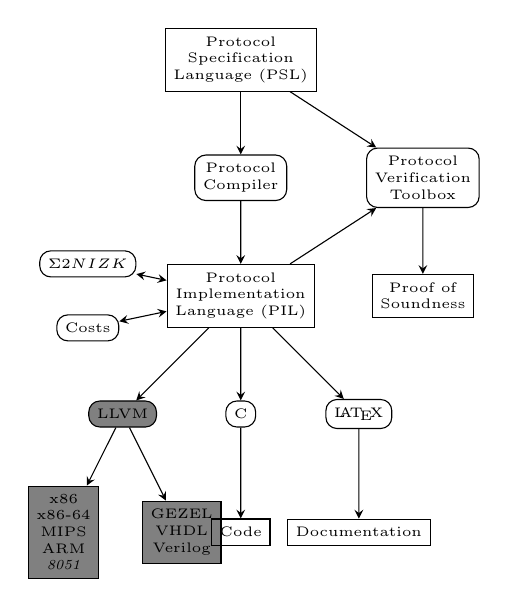
\begin{tikzpicture}[>=stealth]
    \tikzstyle{edge from parent}=[draw,->]
    \node[language] (psl) {Protocol \\ Specification \\ Language (PSL)}
     child {node[compiler] (pc) {Protocol \\ Compiler}
        child {node[language] (pil) {Protocol \\ Implementation \\ Language (PIL)}
            child {node[compiler,added] (llvm) {LLVM}
              child {node[language,added] (asm) {x86 \\ x86-64 \\ MIPS \\ ARM \\ \em{8051}}}
              child {node[language,added] (gezel) {GEZEL \\ VHDL \\ Verilog}}}
            child {node[compiler] (c) {C}
              child {node[language] (code) {Code}}}
            child {node[compiler] (latex) {\LaTeX}
              child {node[language] (doc) {Documentation}}}
          }};

    \node[compiler] (pvt)         [right=of pc,anchor=west]          {Protocol \\ Verification \\ Toolbox}
    child {node[language] {Proof of \\ Soundness}};

    \node[compiler] (sigma) [left=of pil.north west,anchor=center] {$\Sigma 2 N I Z K$};
    \node[compiler] (cost) [left=of pil.south west,anchor=center] {Costs};

    \draw[<->] (sigma) -- (pil);
    \draw[<->] (cost) -- (pil);

    \draw[->] (psl) -- (pvt);
    \draw[->] (pil) -- (pvt);
  \end{tikzpicture}
  \end{center}
\end{frame}

\begin{frame}
  \frametitle{LLVM}

  \begin{itemize}
  \item A proven compiler framework
  \item Already used by SVA (Secure Virtual Architectures)
  \item Uses in many other fields (e.g. GPU, CPU dynamic translation)
    \begin{itemize}
    \item Guarantees maintenance and optimizations (Linus' Law: ``given enough eyeballs, all bugs are shallow'')
    \end{itemize}
  \item Backends for different architectures (e.g. x86, x86-64, ARM, MIPS)
  \item Uses SSA registers
    \begin{itemize}
    \item DFG easy to extract (HW translation possible)
    \end{itemize}
  \end{itemize}
\end{frame}

\begin{frame}
  \frametitle{GEZEL}
  
  \begin{itemize}
  \item A cycle-based HDL (Hardware Description Language)
    \begin{itemize}
    \item Finite-State-Machine + Datapath (FSMD) model
    \end{itemize}
  \item Cosimulation with embedded cores (ARM, 8051, AVR)
  \item Code generator for VHDL and Verilog
  \item Open source
  \end{itemize}
\end{frame}

\begin{frame}
  \frametitle{Planning $\approx 3$ weeks remaining}
  
  \begin{enumerate}
  \item \textcolor{yellow}{Theoretical study} $\approx 3$ days remaining
    \begin{enumerate}
    \item \textcolor{green}{ZK PoK}
    \item \textcolor{yellow}{DAA} $\approx 3$ days remaining
    \end{enumerate}
  \item \textcolor{green}{Evaluate existing frameworks}
    \begin{enumerate}
    \item \textcolor{green}{Evaluate a sample protocol (Schnorr's)}
    \item \textcolor{green}{Add extensions and couple}
      \begin{itemize}
      \item \textcolor{green}{Add terminal functionality to CACE}
      \item \textcolor{green}{Add terminal functionality to GEZEL}
      \item \textcolor{green}{Implement a dummy prover/verifier in GEZEL}
      \end{itemize}
    \end{enumerate}
  \item \textcolor{yellow}{Implement custom framework} $\approx 1$ week remaining
    \begin{enumerate}
    \item \textcolor{green}{Implement parser to AST (Abstract Syntax Trees)}
    \item \textcolor{yellow}{Implement code-generation to LLVM} $\approx 1$ day remaining
    \item \textcolor{yellow}{Implement a JIT compiler} $\approx 1$ day remaining
    \item \textcolor{red}{Implement an LLVM backend for 8051} $\approx 5$ days remaining
    \end{enumerate}
  \item \textcolor{red}{Implement DAA on top of custom framework} $\approx 3$ days remaining
  \item \textcolor{yellow}{Thesis text and presentation} $\approx 2$ weeks remaining
  \end{enumerate}
\end{frame}

\begin{frame}
  \frametitle{Custom framework status}
  
  \begin{table}
    \centering
    \begin{tabular}{|c|c|}
      \hline
      Arrays             & \cellcolor{red} Not started \\ \hline
      Assignment         & \cellcolor{green} Done \\ \hline
      Conditional        & \cellcolor{yellow} Parser done \\ \hline
      Iteration          & \cellcolor{red} Not started \\ \hline
      Function call      & \cellcolor{green} Done \\ \hline
      Function defintion & \cellcolor{green} Done \\ \hline
      Global variables   & \cellcolor{green} Done \\ \hline
      Local data-flow    & \cellcolor{green} Done \\ \hline
      Return values      & \cellcolor{yellow} Mostly done \\ \hline
      Type inference     & \cellcolor{green} Basic \\
      \hline
    \end{tabular}
  \end{table}
\end{frame}

\begin{frame}
  \frametitle{The End}
  
  \begin{itemize}
  \item Thank you
  \item Questions?
  \end{itemize}
\end{frame}

\end{document}


%%% Local Variables: 
%%% TeX-PDF-mode: t
%%% TeX-master: t
%%% End: 
